\documentclass{beamer}
%
% Choose how your presentation looks.
%
% For more themes, color themes and font themes, see:
% http://deic.uab.es/~iblanes/beamer_gallery/index_by_theme.html
%
\mode<presentation>
{
  \usetheme{default}      % or try Darmstadt, Madrid, Warsaw, ...
  \usecolortheme{default} % or try albatross, beaver, crane, ...
  \usefonttheme{default}  % or try serif, structurebold, ...
  \setbeamertemplate{navigation symbols}{}
  \setbeamertemplate{caption}[numbered]
}

\usepackage[english]{babel}
\usepackage[utf8x]{inputenc}

\usepackage{amstext}
%\usepackage{coloremoji}
\usepackage{layout}
\usepackage{multirow}

\usepackage{graphicx}
\graphicspath{ {figs/} }

\setbeameroption{hide notes}
\setbeamertemplate{note page}[plain]
\usepackage{listings}
\usepackage{datetime}
\usepackage{url}

% specifications for presenter mode
%\beamerdefaultoverlayspecification{<+->}
%\setbeamercovered{transparent}

% math shorthand
\usepackage{bm}
\usepackage{amsmath}
\usepackage{mathtools}
\newcommand{\R}{\mathbb{R}}
\newcommand{\D}{\mathcal{D}}
\newcommand{\E}{\mathbb{E}}
\newcommand{\F}{\mathcal{F}}
\newcommand{\X}{\mathcal{X}}
\newcommand{\lik}{\mathcal{L}}
\DeclarePairedDelimiterX{\infdivx}[2]{(}{)}{%
  #1\;\delimsize\|\;#2%
}
\newcommand{\infdiv}{D\infdivx}
\DeclarePairedDelimiter{\norm}{\lVert}{\rVert}
\DeclareMathOperator*{\argmin}{arg\,min}
\DeclareMathOperator*{\argmax}{arg\,max}

% Bibliography
\usepackage{natbib}
\bibpunct{(}{)}{,}{a}{}{;}
\usepackage{bibentry}

%\nobibliography*
\title[zinbwave-droplasso]{Differential Expression Analysis Techniques for
  Single-Cell RNA-seq Experiments}
\subtitle{\vspace*{0.5em} \scriptsize for the Computational Biology Doctoral
  Seminar (CMPBIO 293),\\ organized by N.~Yosef \& T.~Ashuach, Spring 2018, UC
  Berkeley}
\author{Kevin Benac and Nima Hejazi}
\institute{Group in Biostatistics,\\ University of California, Berkeley}
\date{11 April 2018}

%%%%%%%%%%%%%%%%%%%%%%%%%%%%%%%%%%%%%%%%%%%%%%%%%%%%%%%%%%%%%%%%%%%%%%%%%%%%%%%%

%\setcounter{tocdepth}[2]
\AtBeginSubsection[]{
\begin{frame}{Outline}
\tableofcontents[currentsection,currentsubsection]
\end{frame}
}

%%%%%%%%%%%%%%%%%%%%%%%%%%%%%%%%%%%%%%%%%%%%%%%%%%%%%%%%%%%%%%%%%%%%%%%%%%%%%%%%

\begin{document}

\begin{frame}
  \titlepage
\end{frame}

%%%%%%%%%%%%%%%%%%%%%%%%%%%%%%%%%%%%%%%%%%%%%%%%%%%%%%%%%%%%%%%%%%%%%%%%%%%%%%%%
\section{Introduction}
\subsection{Data (Kevin)}
%%%%%%%%%%%%%%%%%%%%%%%%%%%%%%%%%%%%%%%%%%%%%%%%%%%%%%%%%%%%%%%%%%%%%%%%%%%%%%%%

\begin{frame}{The Data: Single-Cell RNA-seq}

\begin{itemize}
  \itemsep12pt
  \item ...
\end{itemize}

\end{frame}

%%%%%%%%%%%%%%%%%%%%%%%%%%%%%%%%%%%%%%%%%%%%%%%%%%%%%%%%%%%%%%%%%%%%%%%%%%%%%%%%

\begin{frame}{The Data: Single-Cell RNA-seq}

\begin{itemize}
  \itemsep12pt
  \item ...
\end{itemize}

\end{frame}

%%%%%%%%%%%%%%%%%%%%%%%%%%%%%%%%%%%%%%%%%%%%%%%%%%%%%%%%%%%%%%%%%%%%%%%%%%%%%%%%

\begin{frame}{The Data: Single-Cell RNA-seq}

\begin{itemize}
  \itemsep12pt
  \item ...
\end{itemize}

\end{frame}

%%%%%%%%%%%%%%%%%%%%%%%%%%%%%%%%%%%%%%%%%%%%%%%%%%%%%%%%%%%%%%%%%%%%%%%%%%%%%%%%
\subsection{Objective (Nima)}
%%%%%%%%%%%%%%%%%%%%%%%%%%%%%%%%%%%%%%%%%%%%%%%%%%%%%%%%%%%%%%%%%%%%%%%%%%%%%%%%

\begin{frame}{The Objective: Differential Expression}

\begin{itemize}
  \itemsep12pt
  \item Why ``differential''? The goal is to find a subset of relevant
    biomarkers with respect to a particular condition of interest (e.g.,
    disease, tissue of origin).
  \item Many experimental settings seek to isolate a subset of biomarkers from
    the full (larger) assayed set in order to identify biological patterns and
    better inform future biological experiments.
  \item Since experimental costs are high and modern biotechnologies allow
    numerous biological targets (e.g., genes) to be assayed, the result is a
    very high-dimensional statistical problem.
\end{itemize}

\end{frame}

%%%%%%%%%%%%%%%%%%%%%%%%%%%%%%%%%%%%%%%%%%%%%%%%%%%%%%%%%%%%%%%%%%%%%%%%%%%%%%%%

\begin{frame}{The Objective: Differential Expression}

\begin{itemize}
  \itemsep12pt
  \item Regularized Linear Models:
    \[
      \min_{w \in \R^d} \left\{ \frac{1}{n} \sum_{i = 1}^n \lik(w, x_i, y_i) +
        \lambda \Omega(w) \right\}
    \]
  \item Lasso for continuous outcomes (squared-error loss):
    \[
      \min_{w \in \R^d} \left\{ \frac{1}{n} \sum_{i = 1}^n \left(y_i - \sum_{j =
        1}^d w_j x_{i,j} \right)^2 + \lambda \sum_{j = 1}^d \lvert w_j \rvert
        \right\}
    \]
\end{itemize}

\end{frame}

%%%%%%%%%%%%%%%%%%%%%%%%%%%%%%%%%%%%%%%%%%%%%%%%%%%%%%%%%%%%%%%%%%%%%%%%%%%%%%%%
\section{Methodology}
\subsection{ZINB-WaVE (Kevin)}
%%%%%%%%%%%%%%%%%%%%%%%%%%%%%%%%%%%%%%%%%%%%%%%%%%%%%%%%%%%%%%%%%%%%%%%%%%%%%%%%

\begin{frame}{ZINB-WaVE I}

\begin{itemize}
  \itemsep12pt
  \item ...
  \item ...
\end{itemize}

\end{frame}
%%%%%%%%%%%%%%%%%%%%%%%%%%%%%%%%%%%%%%%%%%%%%%%%%%%%%%%%%%%%%%%%%%%%%%%%%%%%%%%%

\begin{frame}{ZINB-WaVE II}

\begin{itemize}
  \itemsep12pt
  \item ...
  \item ...
\end{itemize}

\end{frame}

%%%%%%%%%%%%%%%%%%%%%%%%%%%%%%%%%%%%%%%%%%%%%%%%%%%%%%%%%%%%%%%%%%%%%%%%%%%%%%%%

\begin{frame}{ZINB-WaVE III}

\begin{itemize}
  \itemsep12pt
  \item ...
  \item ...
\end{itemize}

\end{frame}

%%%%%%%%%%%%%%%%%%%%%%%%%%%%%%%%%%%%%%%%%%%%%%%%%%%%%%%%%%%%%%%%%%%%%%%%%%%%%%%%

\begin{frame}{ZINB-WaVE IV}

\begin{itemize}
  \itemsep12pt
  \item ...
  \item ...
\end{itemize}

\end{frame}

%%%%%%%%%%%%%%%%%%%%%%%%%%%%%%%%%%%%%%%%%%%%%%%%%%%%%%%%%%%%%%%%%%%%%%%%%%%%%%%%
\subsection{DropLasso (Nima)}
%%%%%%%%%%%%%%%%%%%%%%%%%%%%%%%%%%%%%%%%%%%%%%%%%%%%%%%%%%%%%%%%%%%%%%%%%%%%%%%%

\begin{frame}{DropLasso I}

\begin{itemize}
  \itemsep12pt
  \item Consider the following data structure:
    \begin{itemize}
      \itemsep10pt
      \item $x_i \in \mathbb{R}^d$ --- design matrix of scRNA-seq counts
      \item $y_i \in \mathbb{R}$ --- cell-level outcome of interest (e.g.,
        tissue of origin)
      \item $\delta_i \in \{0, 1\}^d$ s.t.~$\delta_i \sim Bern(p)^d$ --- random
        dropout mask
      \item $\delta \odot x \in \mathbb{R}^d$ --- corrupted pattern for
        scRNA-seq dropout
      \item $\text{P}(\delta_i = 1) = \text{p}$ --- probability of \textit{not}
        being censored by dropout
    \end{itemize}
  \item The DropLasso procedure seeks to identify differentially expressed genes
    based on cell-level differences while accounting for the dropout noise that
    masks scRNA data.
\end{itemize}

\end{frame}

%%%%%%%%%%%%%%%%%%%%%%%%%%%%%%%%%%%%%%%%%%%%%%%%%%%%%%%%%%%%%%%%%%%%%%%%%%%%%%%%

\begin{frame}{DropLasso II}

\begin{itemize}
  \itemsep12pt
  \item Introducing dropout ($\delta_i \sim Bern(p)^d$):
    \[
      \min_{w \in \R^d} \left\{ \frac{1}{n} \sum_{i = 1}^n \E_{\delta_i}
        \lik \left(w, \delta_i \odot \frac{x_i}{p}, y_i \right) + \lambda
        \lVert w \rVert_1 \right\}
    \]
  \item Independence from $p$ in expectation:
    \[
      \begin{aligned}
      \E_{\delta_i} \sum_{j = 1}^{d} w_j \left( \delta_i \odot \frac{x_i}{p}
      \right)_j =& \sum_{j = 1}^d \E_{\delta_i} w_j \delta_{i,j}
      \frac{x_{i,j}}{p} \\ =& \sum_{j = 1}^d w_j x_{i,j}
      \end{aligned}
    \]
\end{itemize}

\end{frame}

%%%%%%%%%%%%%%%%%%%%%%%%%%%%%%%%%%%%%%%%%%%%%%%%%%%%%%%%%%%%%%%%%%%%%%%%%%%%%%%%

\begin{frame}{DropLasso III}

\begin{itemize}
  \itemsep12pt
  \item Introducing the dropout term $\delta$ amounts to censoring the observed
    data and adjusting (i.e., $\frac{x_p}{p}$) such that the effects of dropout
    noise are removed.
  \item This places a \textit{statistical model} on the dropout noise --- i.e.,
    $\delta_i \sim Bern(p)^d$
    \begin{itemize}
      \item Dropout noise is independent across samples and genes. (Fine
        starting point but probably untrue scientifically.)
      \item Modeling dropout noise in a more flexible manner could likely
        improve DropLasso performance and is identified as an item of future
        work.
    \end{itemize}
  \item Merely introducing the simple dropout correction significantly improves
    performance under standard modeling metrics (e.g., AUC).
\end{itemize}

\end{frame}

%%%%%%%%%%%%%%%%%%%%%%%%%%%%%%%%%%%%%%%%%%%%%%%%%%%%%%%%%%%%%%%%%%%%%%%%%%%%%%%%

\begin{frame}{DropLasso IV}

\begin{figure}[H]
  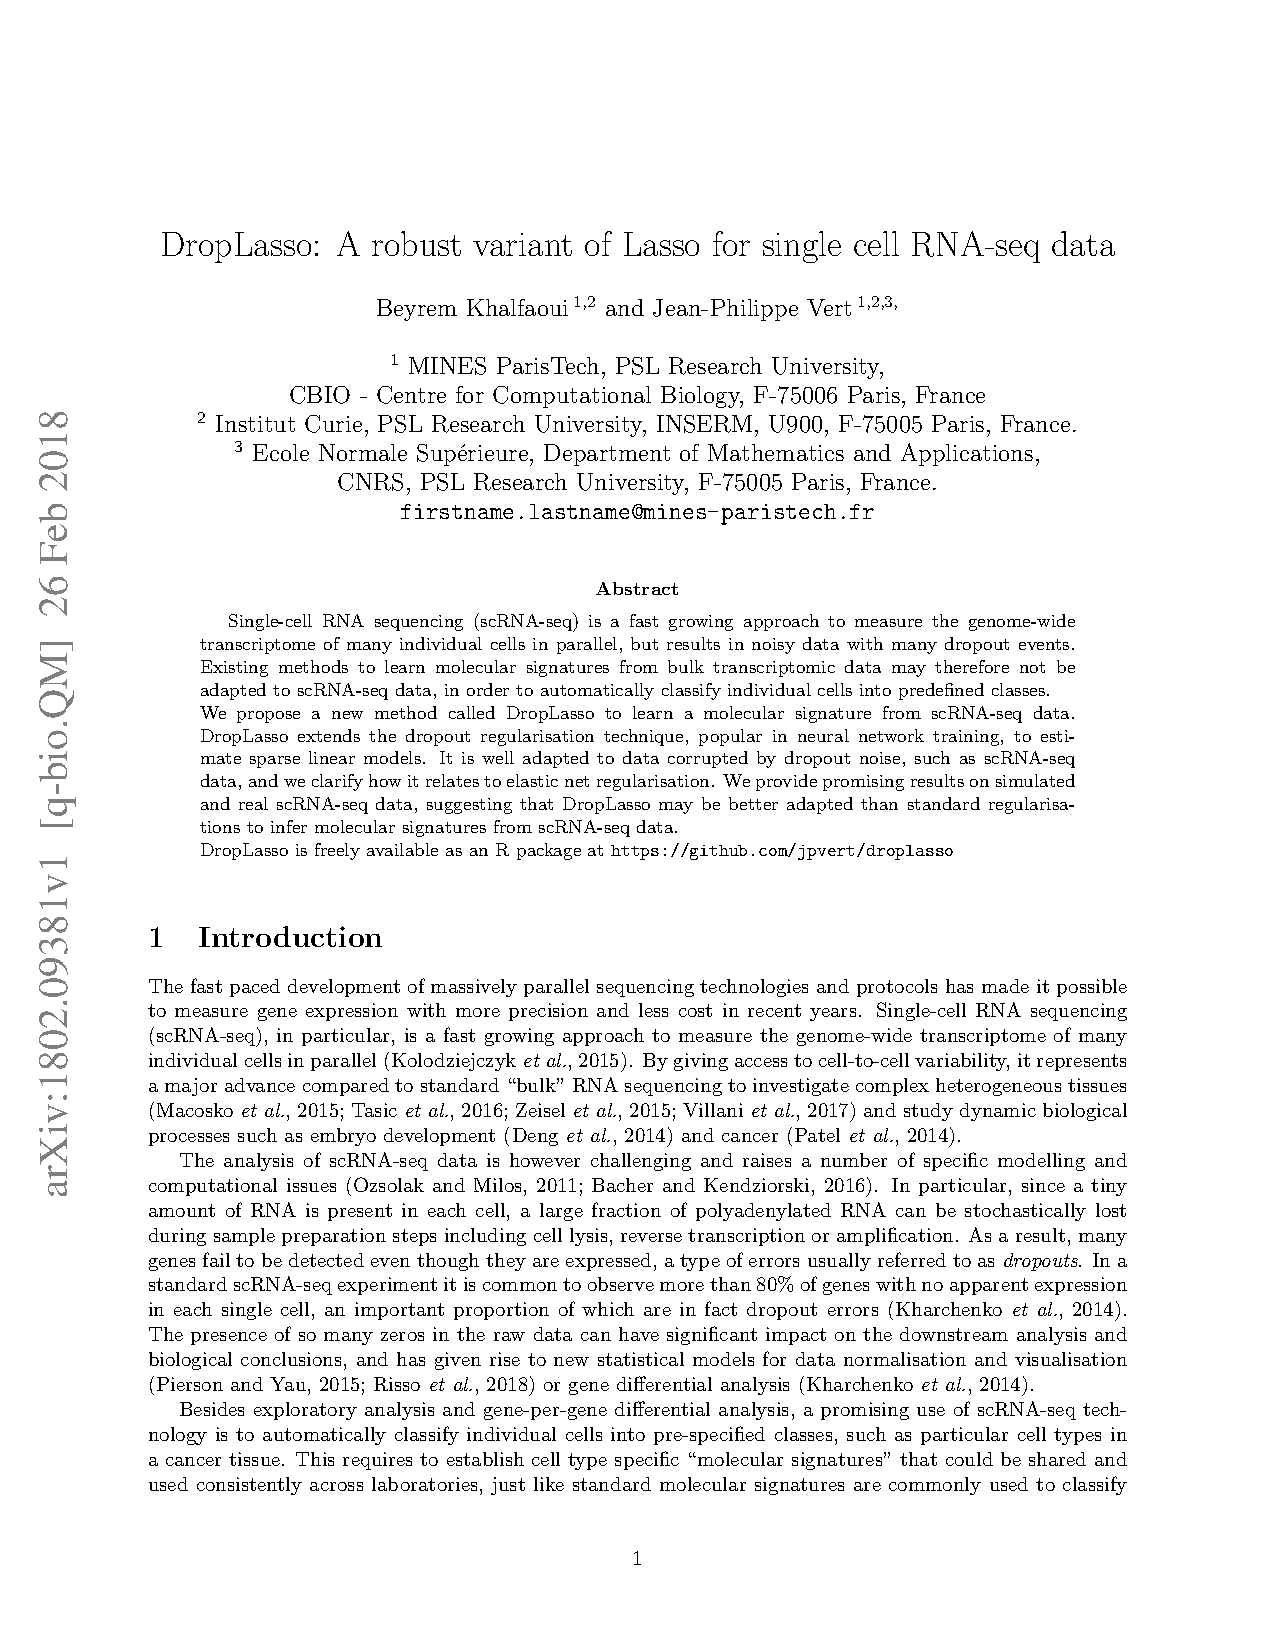
\includegraphics[width=\textwidth]{droplasso}
  \caption{Excerpt from table 3 of ``DropLasso: A robust variant of Lasso for
    single cell RNA-seq data'' Khalfaoui \& Vert (2018)}
\end{figure}

\end{frame}

%%%%%%%%%%%%%%%%%%%%%%%%%%%%%%%%%%%%%%%%%%%%%%%%%%%%%%%%%%%%%%%%%%%%%%%%%%%%%%%%
\subsection{Comparison}
%%%%%%%%%%%%%%%%%%%%%%%%%%%%%%%%%%%%%%%%%%%%%%%%%%%%%%%%%%%%%%%%%%%%%%%%%%%%%%%%

\begin{frame}{ZINB-WaVE v.~DropLasso I}

\begin{itemize}
  \itemsep12pt
  \item ...
  \item ...
\end{itemize}

\end{frame}

%%%%%%%%%%%%%%%%%%%%%%%%%%%%%%%%%%%%%%%%%%%%%%%%%%%%%%%%%%%%%%%%%%%%%%%%%%%%%%%%

\begin{frame}{ZINB-WaVE v.~DropLasso II}

\begin{itemize}
  \itemsep12pt
  \item ...
  \item ...
\end{itemize}

\end{frame}

%%%%%%%%%%%%%%%%%%%%%%%%%%%%%%%%%%%%%%%%%%%%%%%%%%%%%%%%%%%%%%%%%%%%%%%%%%%%%%%%

\begin{frame}{ZINB-WaVE v.~DropLasso III}

\begin{itemize}
  \itemsep12pt
  \item ...
  \item ...
\end{itemize}

\end{frame}

%%%%%%%%%%%%%%%%%%%%%%%%%%%%%%%%%%%%%%%%%%%%%%%%%%%%%%%%%%%%%%%%%%%%%%%%%%%%%%%%
\section{Conclusions}
\subsection{Review}
%%%%%%%%%%%%%%%%%%%%%%%%%%%%%%%%%%%%%%%%%%%%%%%%%%%%%%%%%%%%%%%%%%%%%%%%%%%%%%%%

\begin{frame}{Review}

\begin{itemize}
  \itemsep12pt
  \item ...
  \item ...
\end{itemize}

\end{frame}

%%%%%%%%%%%%%%%%%%%%%%%%%%%%%%%%%%%%%%%%%%%%%%%%%%%%%%%%%%%%%%%%%%%%%%%%%%%%%%%%

% don't want dimming with references
\setbeamercovered{}
\beamerdefaultoverlayspecification{}

\begin{frame}[c,allowframebreaks]{References}

\small
\bibliographystyle{plainnat}
\nocite{*}
\bibliography{refs}
\itemize

\end{frame}

%%%%%%%%%%%%%%%%%%%%%%%%%%%%%%%%%%%%%%%%%%%%%%%%%%%%%%%%%%%%%%%%%%%%%%%%%%%%%%%%

\end{document}

